\documentclass[a4paper]{article}
\usepackage{amsmath}
\usepackage{amssymb}
\usepackage{graphicx}
\usepackage{a4wide}
\usepackage{url}
\usepackage{pdfpages}

\usepackage{natbib}
\citestyle{aa}
\bibpunct{(}{)}{;}{a}{}{,}

\newcommand{\mytilde}{\raise.17ex\hbox{$\scriptstyle\mathtt{\sim}$}}
\setlength{\parindent}{0pt}

% Listings to import code into LaTeX
\usepackage{listings}
\usepackage{color}
\usepackage{textcomp}
\definecolor{listinggray}{gray}{0.9}
\definecolor{lbcolor}{rgb}{0.9,0.9,0.9}
\lstset{
	backgroundcolor=\color{lbcolor},
	tabsize=4,
	rulecolor=,
	language=bash,
        basicstyle=\scriptsize,
        upquote=true,
        aboveskip={1.5\baselineskip},
        columns=fixed,
        showstringspaces=false,
        extendedchars=true,
        breaklines=true,
        prebreak = \raisebox{0ex}[0ex][0ex]{\ensuremath{\hookleftarrow}},
        frame=single,
        showtabs=false,
        showspaces=false,
        showstringspaces=false,
        identifierstyle=\ttfamily,
        keywordstyle=\color[rgb]{0,0,1},
        commentstyle=\color[rgb]{0.133,0.545,0.133},
        stringstyle=\color[rgb]{0.627,0.126,0.941},
}
% End of Listings

\begin{document}
\begin{figure}[h!]
\begin{center}

\includegraphics{UvA_Logo_Image_EN.jpg} \\

\includegraphics{UvA_Logo_Text_EN.jpg} \\

\includegraphics{API_Logo_Text.pdf}
\end{center}
\end{figure}

\begin{center}
\line(1,0){420} \\
\huge \textbf{Computational Astrophysics (CA) \\
Simulating Ultra Compact Dwarf Galaxies with AMUSE} \\
\line(1,0){420}
\end{center}

\vfill

%\begin{figure}[h!]
%\begin{center}
%\includegraphics[width=12cm]{graphgraphMyGraph}
%\end{center}
%\end{figure}
%\addtocounter{figure}{-1} % start counting at figure 1 again


\begin{table}[h]
\begin{center}
\begin{tabular}{lp{5cm}l}
\textit{Author:} & & \emph{Supervisor:} \\
Timo Halbesma, 1603221 & & Prof.dr. S.F. Portegies Zwart\\
Shabaz Sultan, 161745 & & Edwin van der Helm, MSc\\
\end{tabular}
\end{center}
\end{table}

% End of titlepage

\newpage

\abstract{Using the AMUSE framework we have analysed the force calculation N-body algorithms BHTree, Hermite and Huayno. After carefull considerations we found that the BHTree algorithm provides us with the best time-complexity $O(n \log n)$, compared to $O(n^2)$ for both Hermite and Huayno. Moreover, the timestep has been lowered until a satisfying relative energy error in the order of $\mu J$ has been reached. Having set up the gravity and particle models, we were able to simulate a dwarf galaxy orbiting a black hole.}

%\lstinputlisting[caption={Solution for CA / Gravitational
%Dynamics\label{list:main}}]{../GravitationalDynamics/CA_GD_TLRH_s1603221_SS_s1617451.py}
%
%\lstinputlisting[caption={Solution for CA / Gravitational
%Dynamics\label{list:plotter}}]{../GravitationalDynamics/plot_nbody.py}
%
%\lstinputlisting[caption={Solution for CA / Gravitational
%Dynamics\label{list:solver}}]{../GravitationalDynamics/solve_nbody.py}

\newpage

\section*{Assignment 1A}
For all assignments we have made use of the AMUSE framework \citep{2013CoPhC.183..456P, 2013A&A...557A..84P, 2009NewA...14..369P}. In Figure~\ref{fig:BHTree_runtime} and Figure~\ref{fig:BHTree_dE} respectively Figure~\ref{fig:Hermite_runtime} and Figure~\ref{fig:Hermite_dE} the required plots for this assignment can be found. Since the assignment was ambiguous about the algorithm to use (either BHTree \citep{1986Natur.324..446B} or Hermite \citep{1995ApJ...443L..93H}), we considered both. \\

\noindent \textbf{BHTree} \\
The cluster size $r$ is passed to the nbody\_integrator function as parameter
named `rcl'. This parameter is only used in amuse.units.nbbody\_system, which is
responsible for the creation of bodies within a convined cluster with half-mass
radius `rcl'. The distance between individual particles could increase  as the
cluster half mass radius increases. This maximum distance between particles
scales linearly with the cluster half mass radius. The distance between
particles can be found in the force, but the number of times the force is
calculated does not depend on it. If the cluster size increases and the number
of paricles is unchanged, then at a certain point in time more particles could
be further away. In that case more particles will be bundles together in the
same BHTree, thus, in principle the calculation time could decrease as the
cluster size r increases if particles move further away. 

\begin{figure}[h!]
\begin{center}
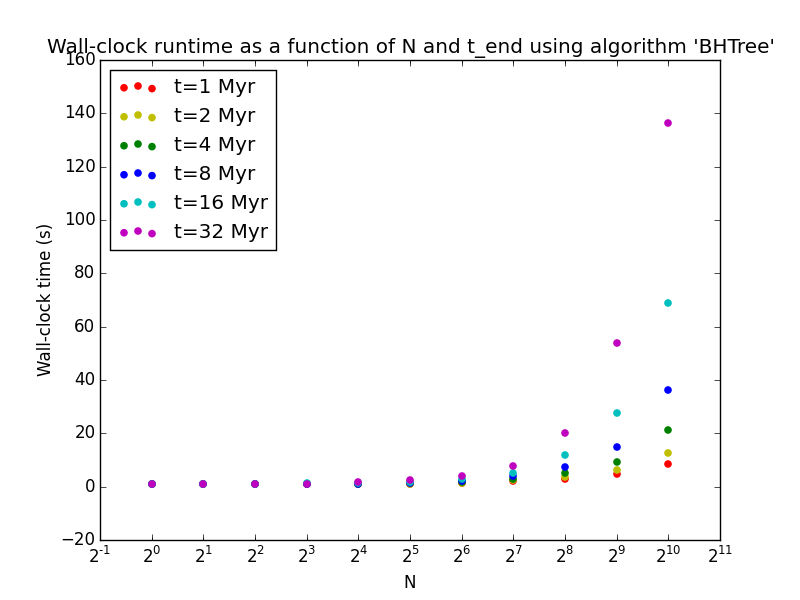
\includegraphics[height=12cm]{../GravitationalDynamics/plots/CA_GD_TLRH_s1603221_SS_s1617451_BHTree_runtime.png}
\caption{Wall-clock time as a function of both N and integration end time for BHTree.}
\label{fig:BHTree_runtime}
\end{center}
\end{figure}

\begin{figure}[h!]
\begin{center}
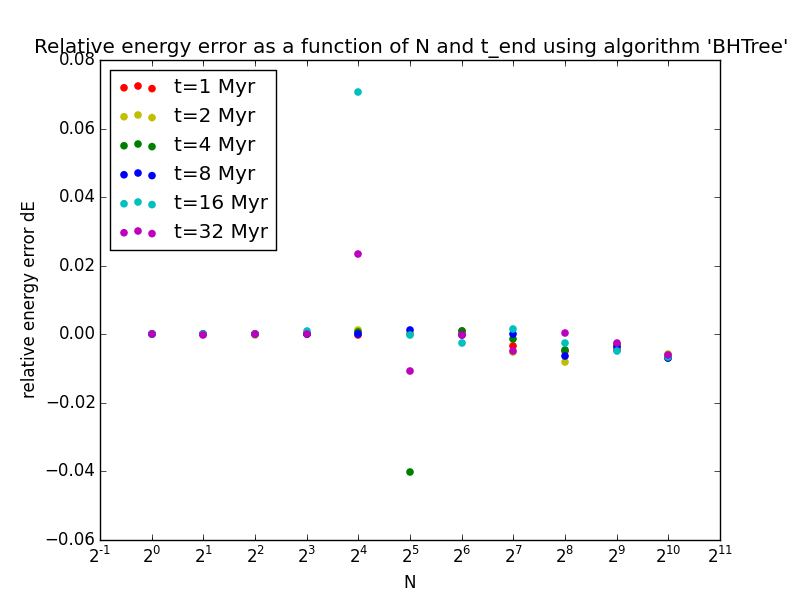
\includegraphics[height=12cm]{../GravitationalDynamics/plots/CA_GD_TLRH_s1603221_SS_s1617451_BHTree_dE.png}
\caption{Relative energy error as a function of both N and integration end time for BHTree.}
\label{fig:BHTree_dE}
\end{center}
\end{figure}

\noindent \textbf{Hermite} \\

\begin{figure}[h!]
\begin{center}
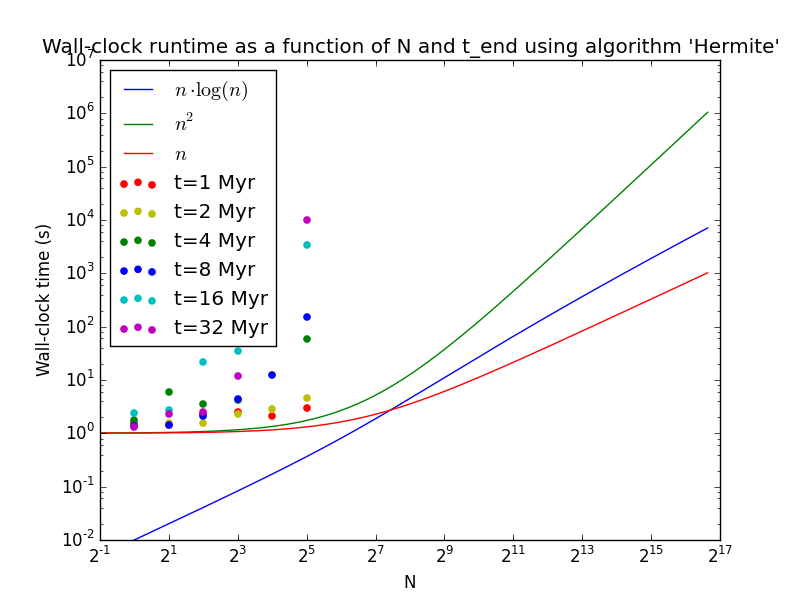
\includegraphics[height=12cm]{../GravitationalDynamics/plots/CA_GD_TLRH_s1603221_SS_s1617451_Hermite_runtime.png}
\caption{Wall-clock time as a function of both N and integration end time for Hermite.}
\label{fig:Hermite_runtime}
\end{center}
\end{figure}

\begin{figure}[h!]
\begin{center}
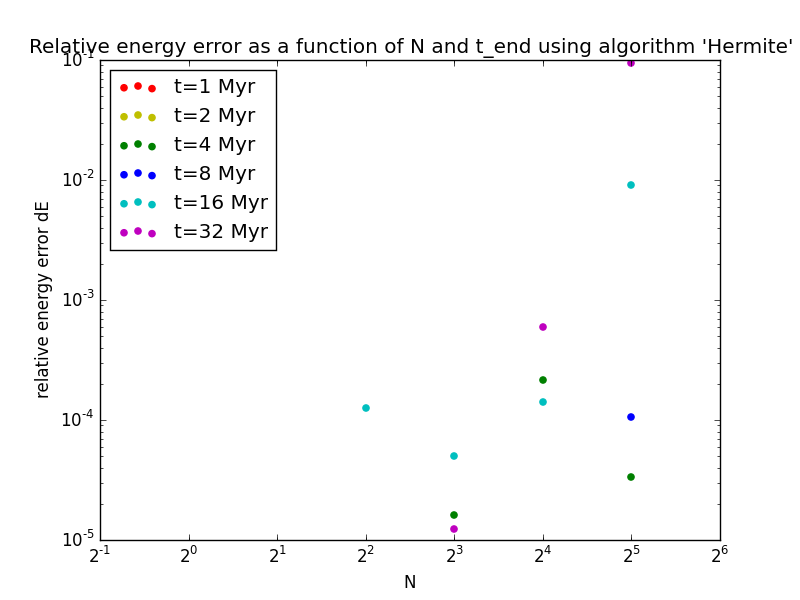
\includegraphics[height=12cm]{../GravitationalDynamics/plots/CA_GD_TLRH_s1603221_SS_s1617451_Hermite_dE.png}
\caption{Relative energy error as a function of both N and integration end time for Hermite.}
\label{fig:Hermite_dE}
\end{center}
\end{figure}

\section*{Assignment 1B} 
HOP \citep{1998ApJ...498..137E}

\section*{Assignment 1C}
In addition to the algorithms considered for assignment~1a, we also used Huayno \citep{2012NewA...17..711P} for analysis.

\begin{figure}[h!]
\begin{center}
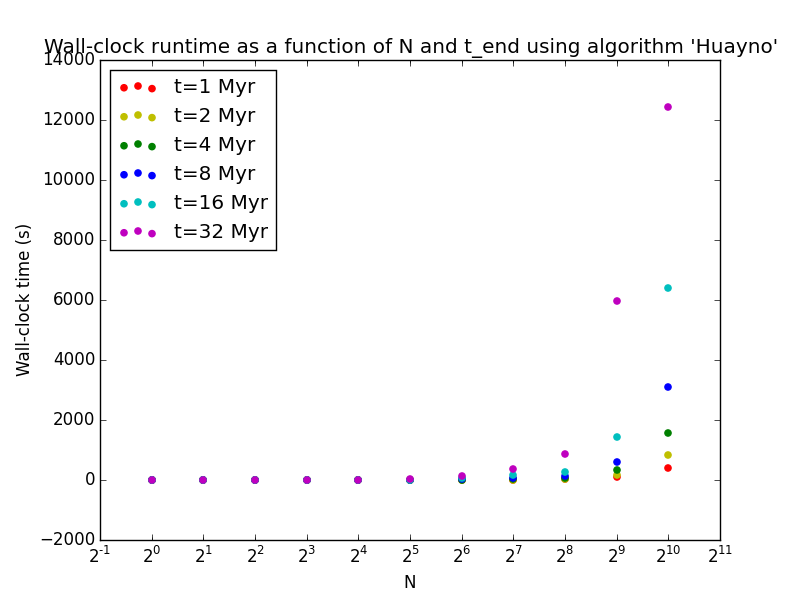
\includegraphics[height=12cm]{../GravitationalDynamics/plots/CA_GD_TLRH_s1603221_SS_s1617451_Huayno_runtime.png}
\caption{Wall-clock time as a function of both N and integration end time for Huayno.}
\label{fig:Huayno_runtime}
\end{center}
\end{figure}

\begin{figure}[h!]
\begin{center}
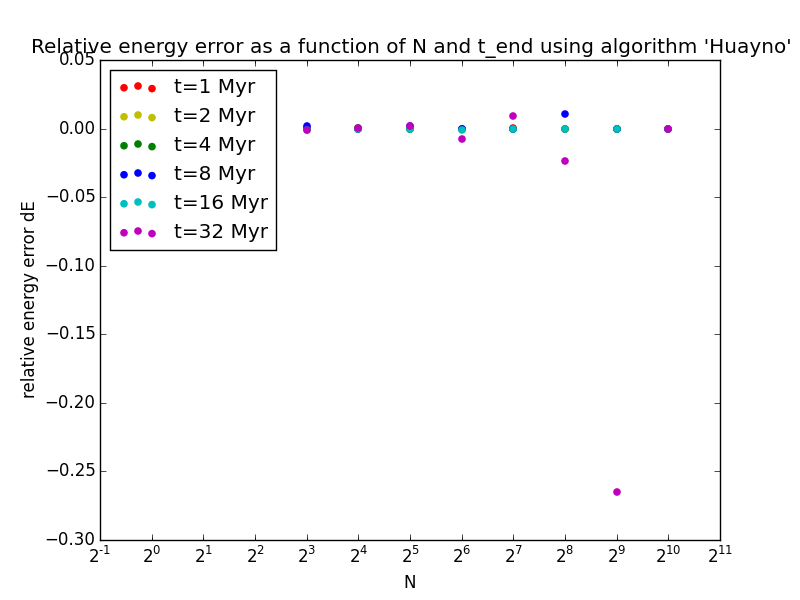
\includegraphics[height=12cm]{../GravitationalDynamics/plots/CA_GD_TLRH_s1603221_SS_s1617451_Huayno_dE.png}
\caption{Relative energy error as a function of both N and integration end time for Huayno.}
\label{fig:Huayno_dE}
\end{center}
\end{figure}

\section*{Assignment 1D}

\section*{Assignment 1E}

\section*{Assignment 1F}

\newpage
\bibliographystyle{apj} 
%\setlength{\bibsep}{0pt} % Remove whitespace in bibliography.
\bibliography{apj-jour,CA_GD_TLRH_s1603221_SS_s1617451_report} 
% \citep{label01}, verwijzing stijl: (Naam 0000) (naam en jaartal).
% \citet{label01} verwijzing stijl Naam (0000), naam en (jaartal).

\end{document}
